\documentclass{article}
\usepackage{amsmath, amssymb, amsfonts, bm}
\usepackage{geometry}
\usepackage{tikz}
\usetikzlibrary{arrows.meta}
\usepackage{float}	
\usepackage{graphicx}
\usepackage[colorlinks = true, allcolors = blue]{hyperref}
\usepackage{algorithm}
\usepackage{algpseudocode}
\usepackage{caption}
\usepackage{color}
\usepackage{soul}
\setlength{\parindent}{0em} 		% remove the indent for all paragraphs
\newcommand{\bl}[1]{\textcolor[rgb]{0.00,0.00,1.00}{#1}}
\newcommand{\gr}[1]{\textcolor[rgb]{0.00,0.50,0.00}{#1}}
\newcommand{\rd}[1]{\textcolor[rgb]{0.75,0.00,0.00}{\st{#1}}}
\newcommand{\tl}[1]{\textcolor[rgb]{0,0.6,0.60}{#1}}
\usepackage[textsize = tiny]{todonotes}
\geometry{a4paper, margin = 1in}

\usepackage{titlesec}
\titleformat{\section}{\normalfont\large\bfseries}{\thesection}{1em}{}
\titleformat{\subsection}{\normalfont\normalsize\bfseries}{\thesubsection}{1em}{}
\titleformat{\subsubsection}{\normalfont\normalsize\bfseries}{\thesubsubsection}{1em}{}

\begin{document}
	
	\title{Step-by-Step Abaqus Modeling of a 2D Shell Beam}
	\author{}
	\date{}
	\maketitle
	
	This document...
	
	\section{Part}
	\underline{Create Part}: Name  =  Part-1; 3D; Deformable; Shell; Extrude\\
	Sketch: 0.089 (m) wide; See Figure [\ref{fig:extsketch}]\\
	Extrude: 0.0254 (m) depth; See Figure [\ref{fig:extsketch}]
	\begin{figure}[H]
		\centering
		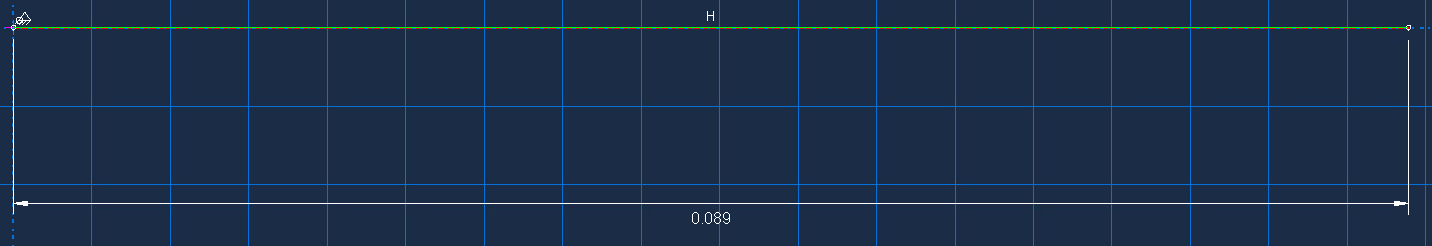
\includegraphics[width =4in]{Figures/shell_extrude_sketch.png}
		\caption{}
		\label{fig:extsketch}
	\end{figure}
	\begin{figure}[H]
		\centering
		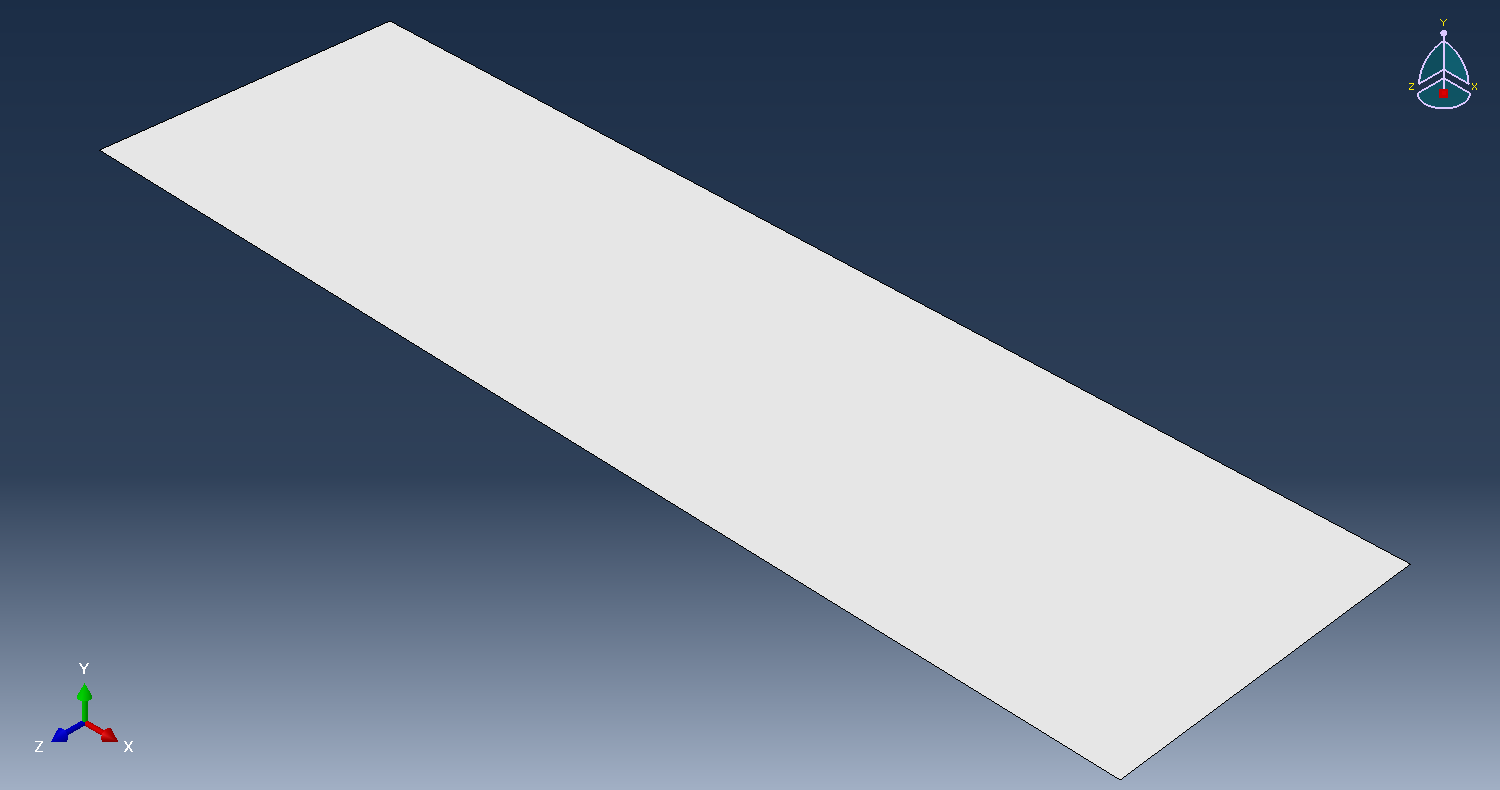
\includegraphics[width=4in]{Figures/shell_extrude.png}
		\caption{}
		\label{fig:ext}
	\end{figure}
	
	\underline{Create Partition}: Face; Sketch; See Figures [\ref{fig:partitionsketch}, \ref{fig:partition}]	
	\begin{figure}[H]
		\centering
		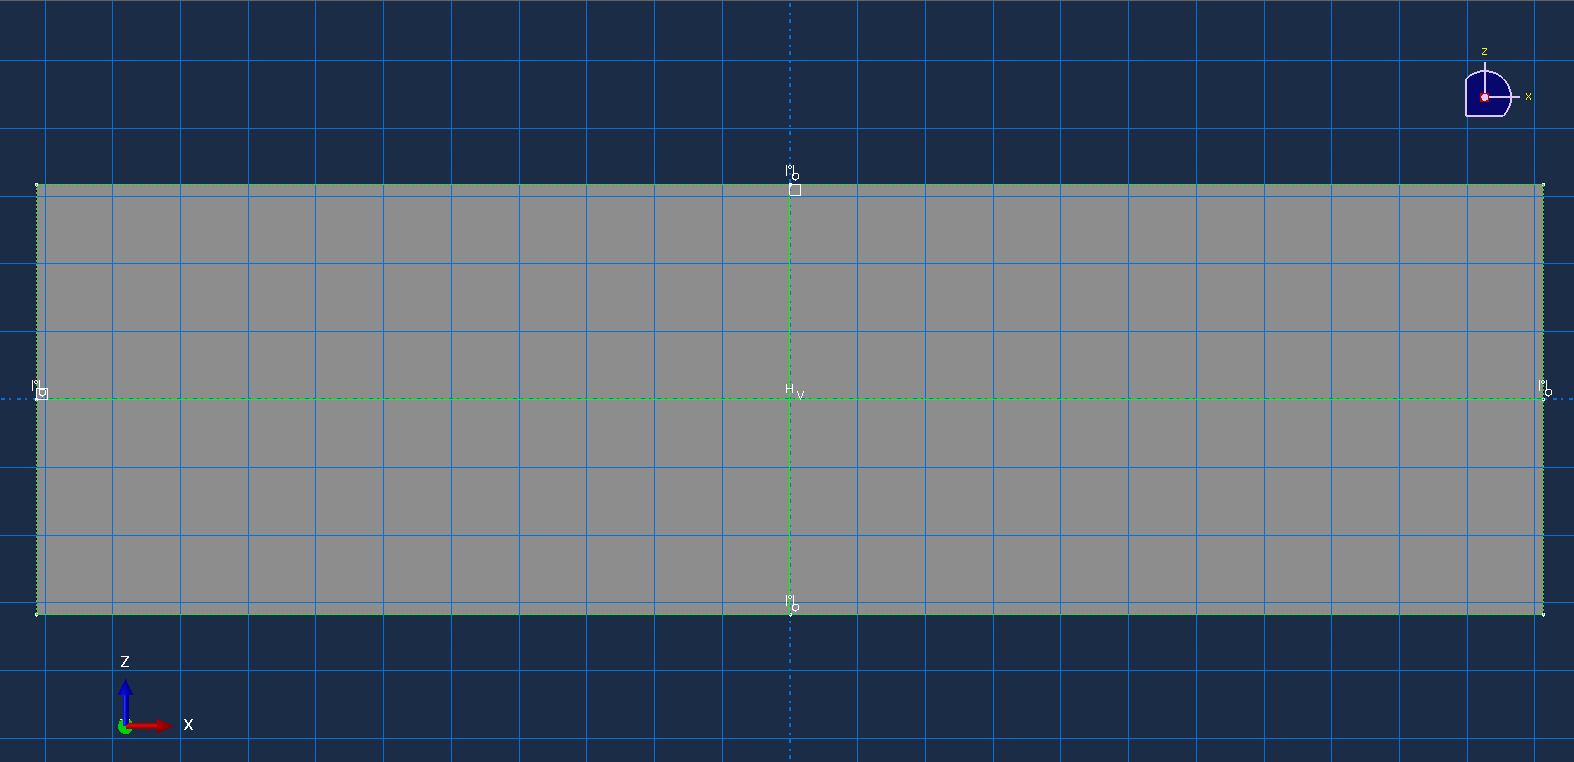
\includegraphics[width=4in]{Figures/partition_sketch.png}
		\caption{Draws lines halfway both long- and short-ways.}
		\label{fig:partitionsketch}
	\end{figure}
	\begin{figure}[H]
		\centering
		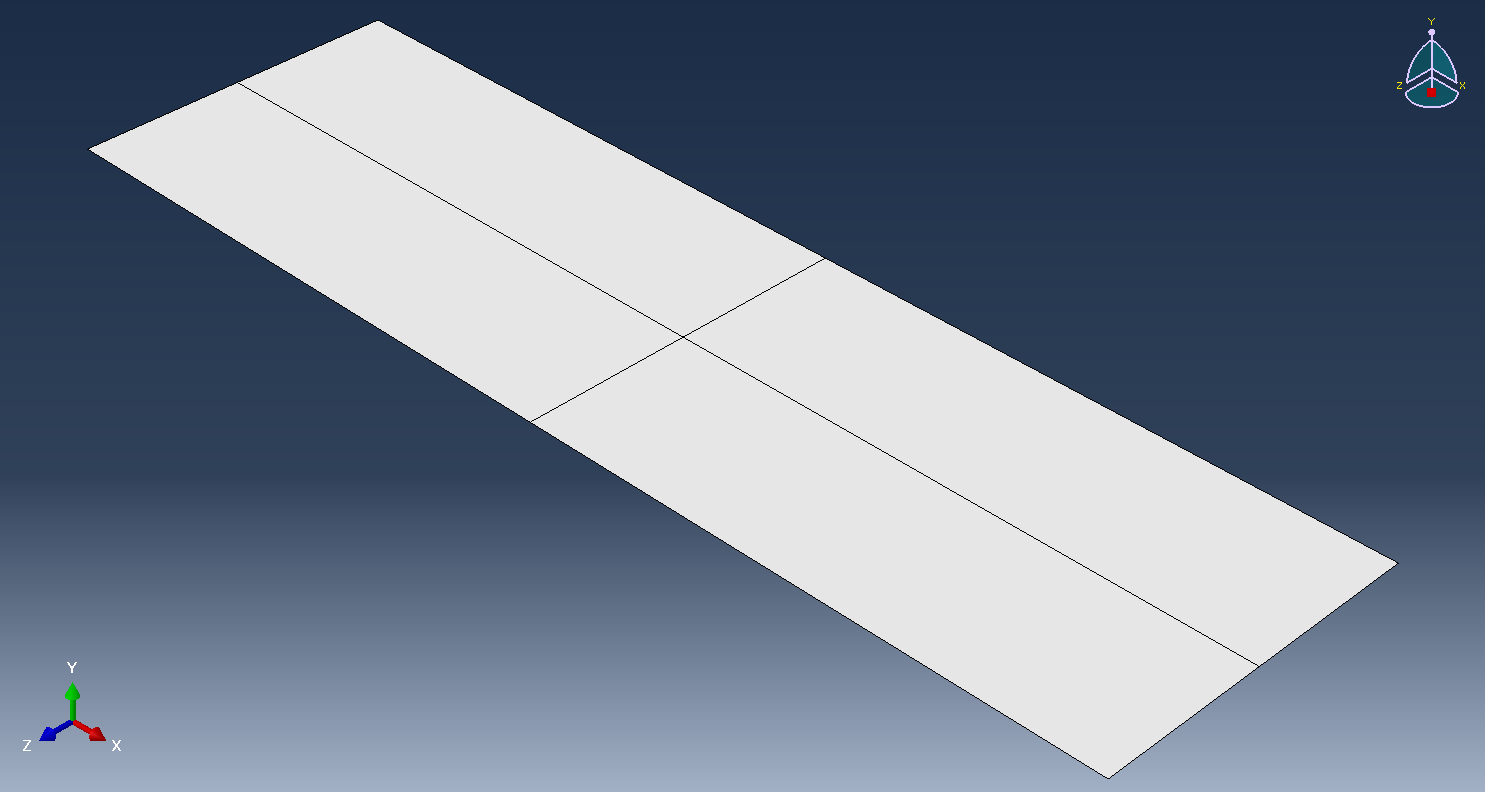
\includegraphics[width=4in]{Figures/partition.png}
		\caption{This creates a partition at the center of the part.}
		\label{fig:partition}
	\end{figure}
	
	\underline{Create Set}: Name = Set-1; See Figure [\ref{fig:set1}]
	\begin{figure}[H]
		\centering
		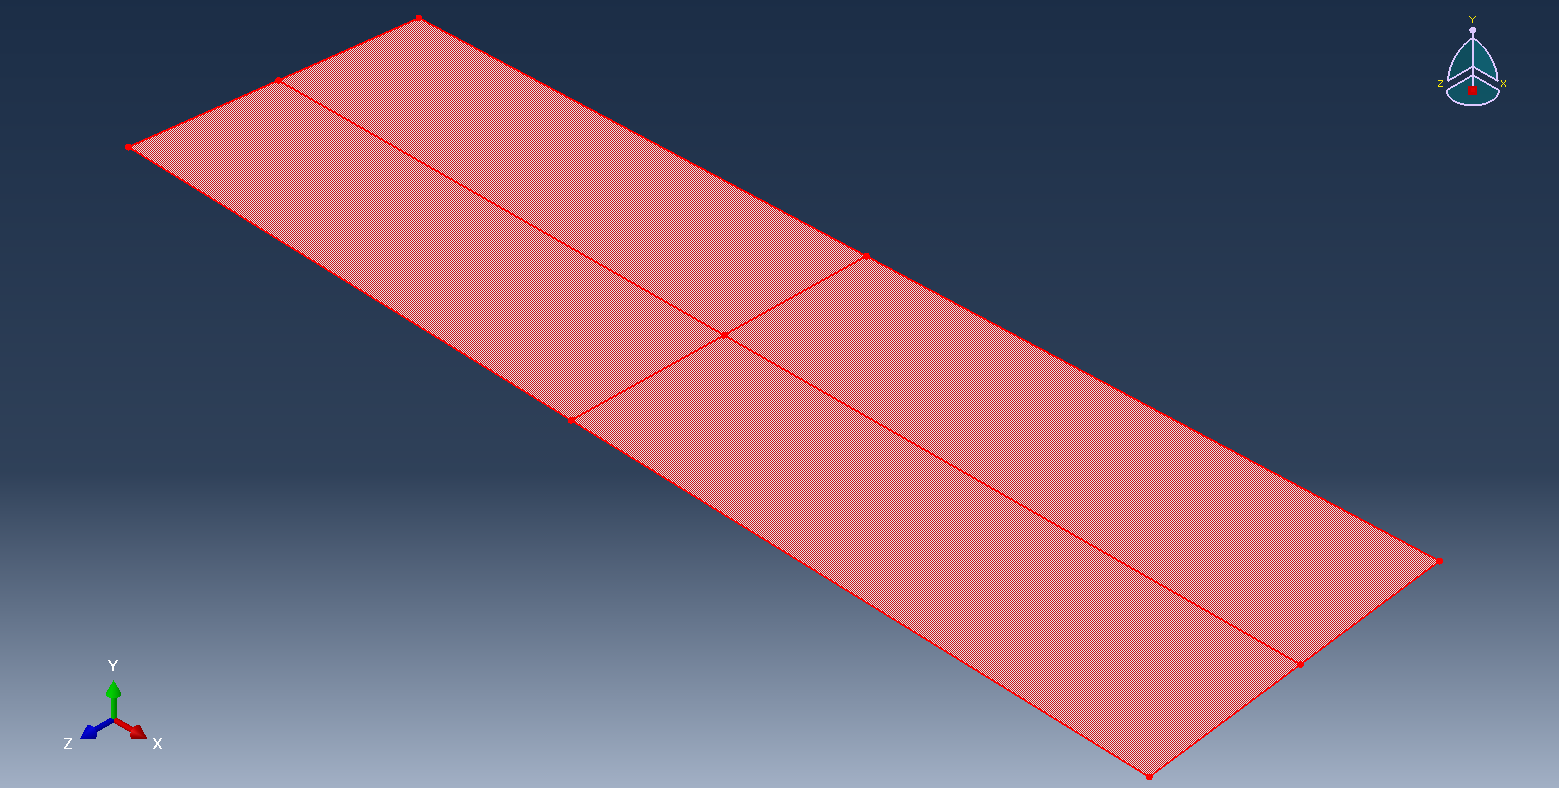
\includegraphics[width=4in]{Figures/set1.png}
		\caption{Select the entire body.}
		\label{fig:set1}
	\end{figure}
	
	\underline{Create Set}: Name = CenterNode; See Figure [\ref{fig:CenterNode}]
	\begin{figure}[H]
		\centering
		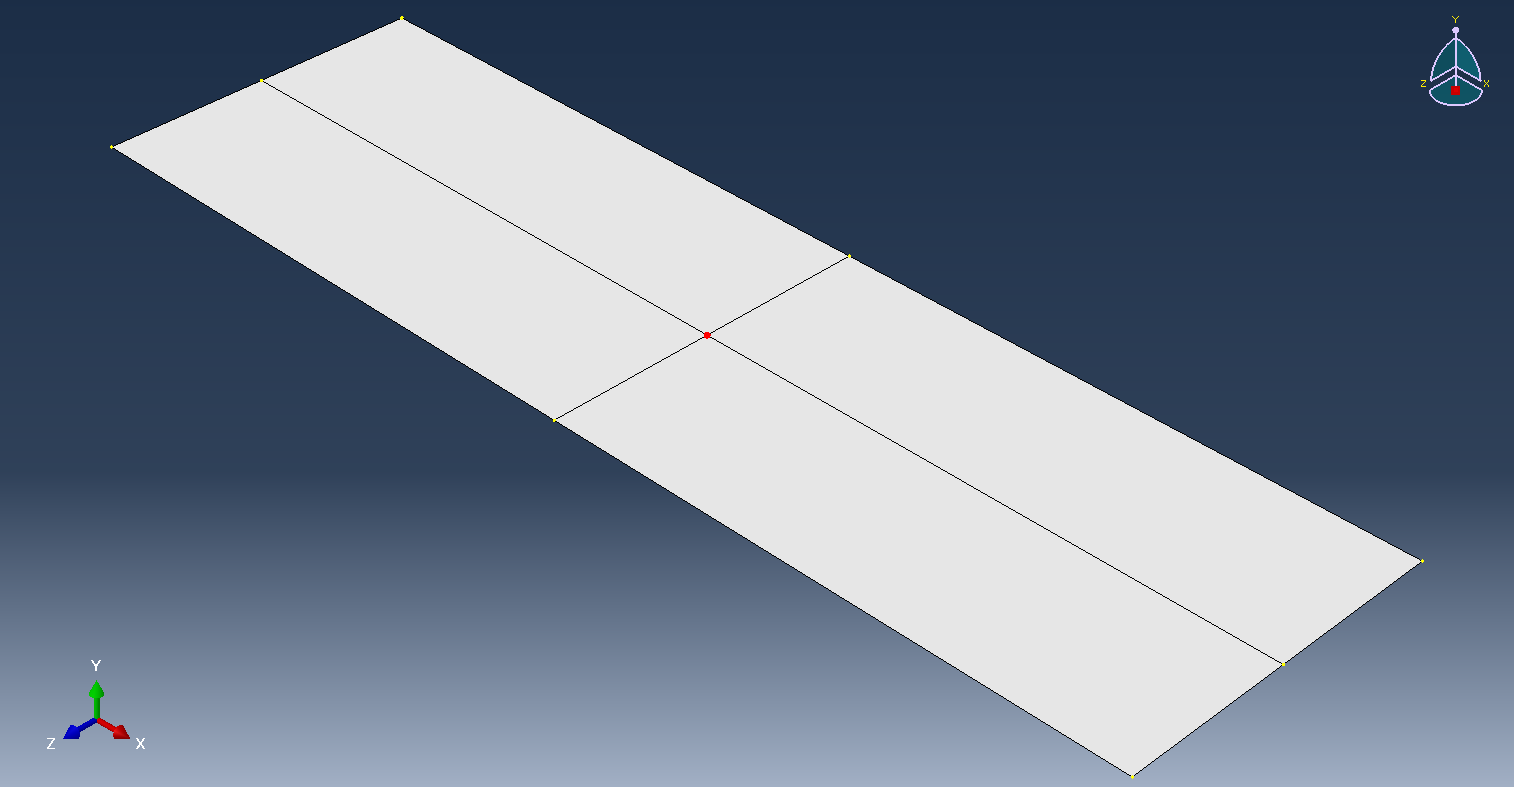
\includegraphics[width=4in]{Figures/CenterNode.png}
		\caption{Select the point at the center of the created partition.}
		\label{fig:CenterNode}
	\end{figure}
	
	\section{Mesh}
	\underline{Seed Part}: Approximate global size = 0.002\\
	Curvature control, Maximum deviation factor = 0.1\\
	Minimum size control, By fraction of global size = 0.1\\
	
	Select Mesh Part; See Figure [\ref{fig:mesh}]
	\begin{figure}[H]
		\centering
		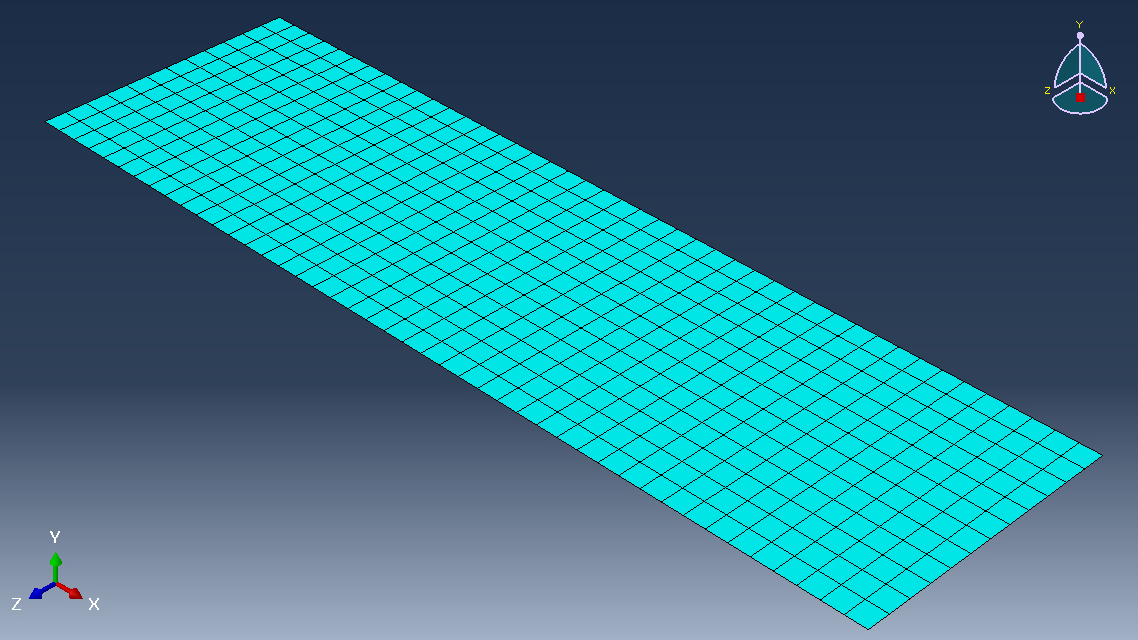
\includegraphics[width=4in]{Figures/mesh.png}
		\caption{}
		\label{fig:mesh}
	\end{figure}
	
	\section{Material}
	\underline{Create Material}: Name = FR4;\\
	General, Density, Mass Density = 1900 (kg/m$^3$)\\
	Mechanical, Elastic, Young's Modulus = 18.6e9; Poisson's Ratio = 0.136\\
	%Samuel used Young's Modulus = 21e9; Poisson's Ratio = 0.136\\
	Mechanical, Damping, Alpha = 65.53; Beta = 3.95e-6
	
	\section{Section}
	\underline{Create Section}: Name = Section-2; Shell; Homogeneous\\
	Section integration = During Analysis; Shell thickness, Value = 0.0016\\
	Material = FR4; Thickness integration rule = Simpson; Thickness integration points = 5
	
	\section{Assembly}
	\underline{Create Instance}: Auto; Parts; Parts = Part-1; See Figure [\ref{fig:instance}]
	\begin{figure}[H]
		\centering
		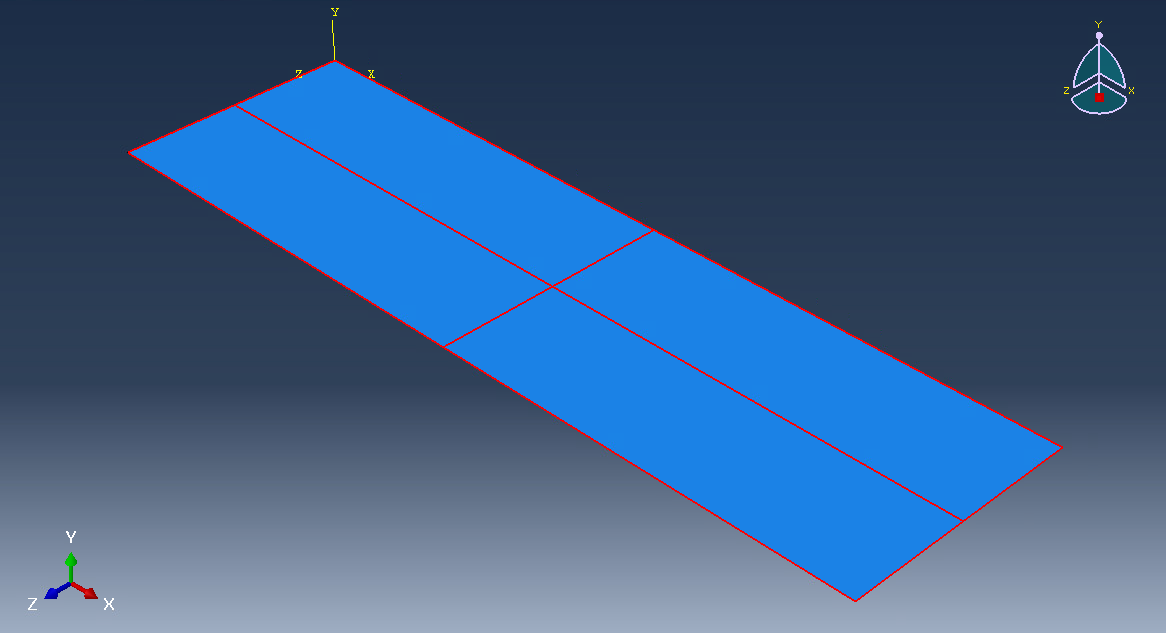
\includegraphics[width=4in]{Figures/instance.png}
		\caption{}
		\label{fig:instance}
	\end{figure}
	
	\underline{Create Set}: Name = Set-1; See Figure [\ref{fig:instance_set1}]
	\begin{figure}[H]
		\centering
		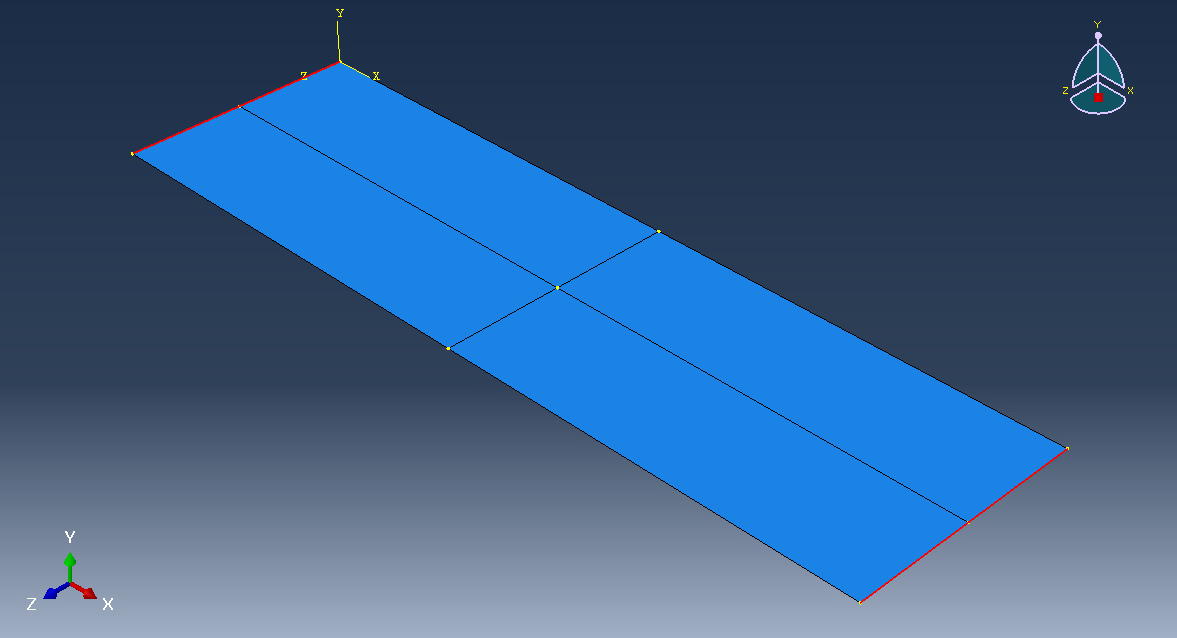
\includegraphics[width=4in]{Figures/instance_set1.png}
		\caption{Select the the edges at the ends of the beam.}
		\label{fig:instance_set1}
	\end{figure}
	
	\underline{Create Set}: Name = Set-2; See Figure [\ref{fig:instance_set2}]
	\begin{figure}[H]
		\centering
		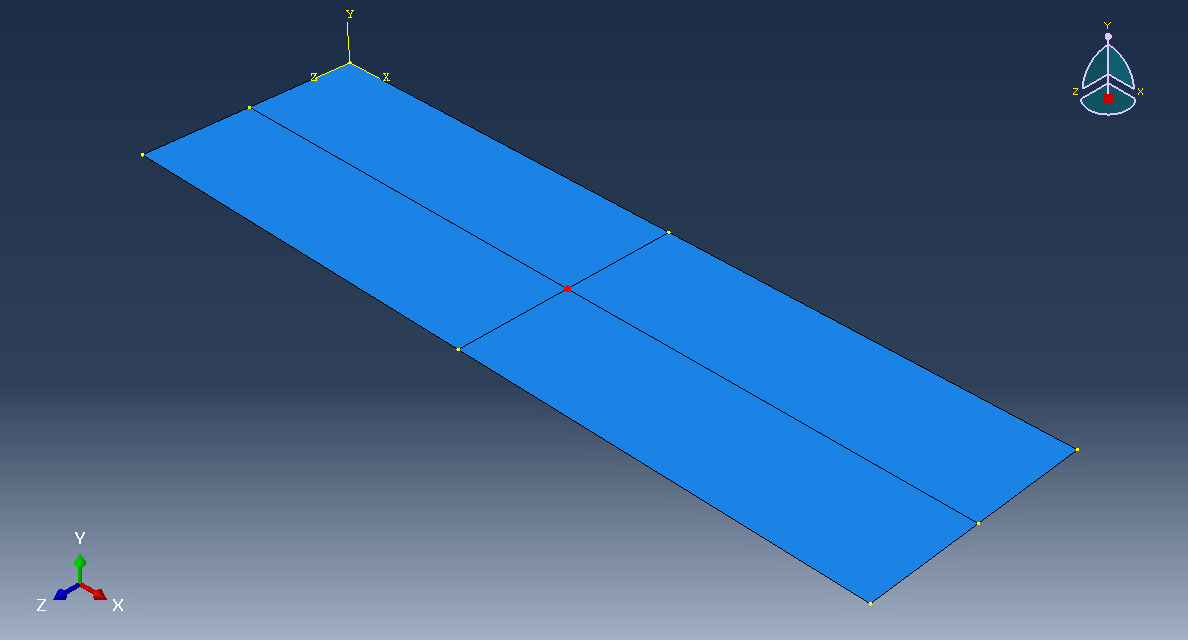
\includegraphics[width=4in]{Figures/instance_set2.png}
		\caption{Select the point at the center.}
		\label{fig:instance_set2}
	\end{figure}
	
	\section{Step}
	\underline{Create Step}: Name = Force; Insert new step after Initial; General; Dynamic, Explicit\\
	Under Basic: Time period = 0.05\\
	Under Incrementation: Automatic; Global; Improved Dt Method; Unlimited; Time scaling factor = 1
	
	\section{Amplitude/Load}
	\underline{Create Amplitude}: Tabular; Step time; Use solver default; See Table [\ref{tab:amplitude}]
	
	\begin{table}[H]
		\centering
		\caption{Under Amplitude Data}
		\label{tab:amplitude}
		\begin{tabular}{|c|c|c|}
			\hline
			 & Time/Frequency & Amplitude\\ \hline
			1 & 0 & 0 \\ %\hline
			2 & 0.005 & 0 \\ %\hline
			3 & 0.005001 & 1\\ %\hline
			4 & 0.0051 & 1\\ %\hline
			5 & 0.005101 & 0\\ \hline
		\end{tabular}
	\end{table}
	
	\underline{Create Load}: Name = Load-1; Step = Force; Mechanical; Concentrated Force; Region = Set-2\\
	Distribution = Uniform; CF1 = 0; CF2 = -30; CF3 = 0; Amplitude = Amp-3; See Figure [\ref{fig:load1}]
	\begin{figure}[H]
		\centering
		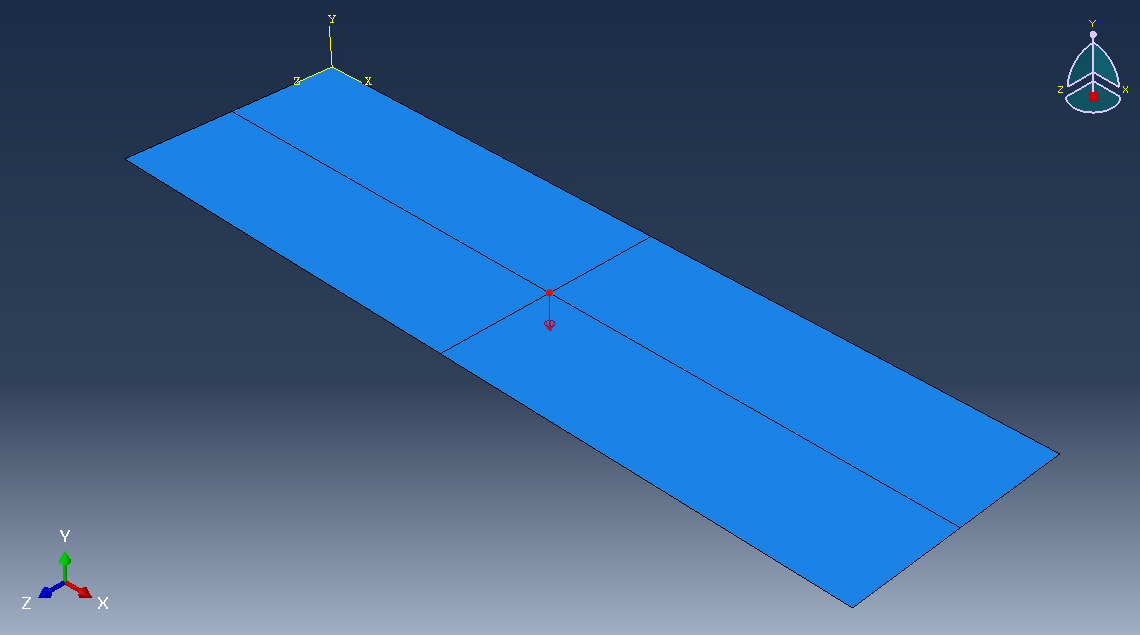
\includegraphics[width=4in]{Figures/load1.png}
		\caption{}
		\label{fig:load1}
	\end{figure}
	
	\section{Boundary Conditions}
	\underline{Create BC}: Name = FixedEnds; Step = Initial; Mechanical; Symmetry/Antisymmetry/Encaste\\
	Select Set-1; ENCASTE (U1 = U2 = U3 = UR1 = UR2 = UR3 = 0); See Figure [\ref{fig:fixed_ends}]
	\begin{figure}[H]
		\centering
		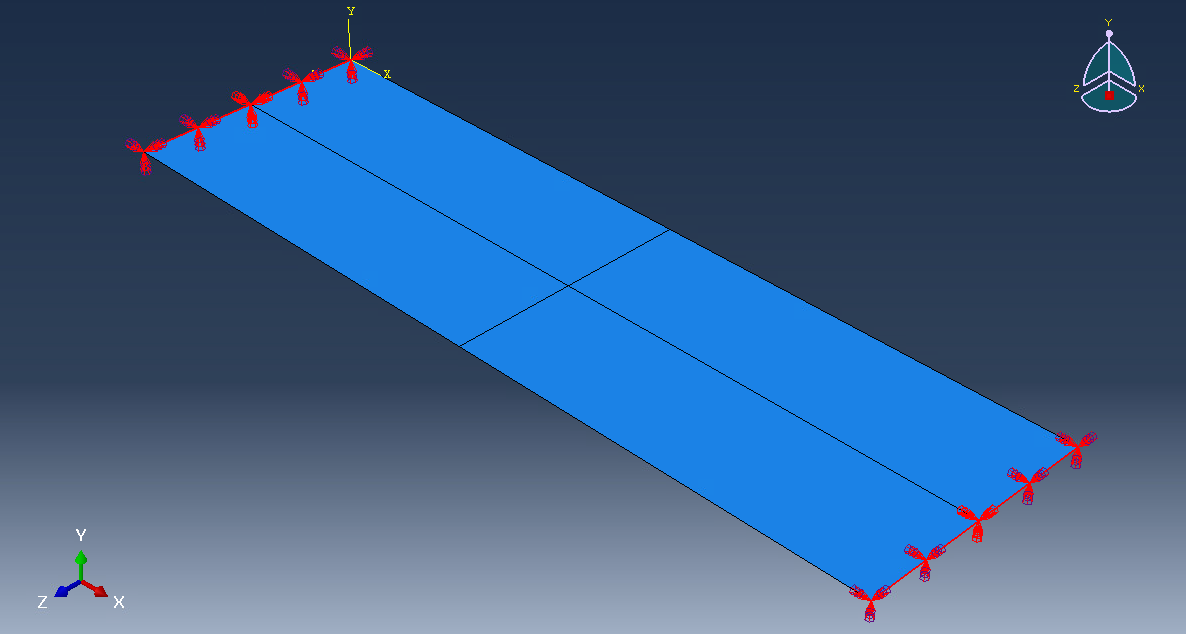
\includegraphics[width=4in]{Figures/fixed_ends.png}
		\caption{}
		\label{fig:fixed_ends}
	\end{figure}
	
	\section{History Output Request}
	\underline{Create History}: Name = CenterDisp; Step = Force\\
	Domain = Set,Part-1-1.CenterNode; Frequency = Evenly spaced time intervals; Interval = 200\\
	Under Output Variables: [Select from list below, Displacement/Velocity/Acceleration] U, Translations and rotations\\
	Use defaults; Use global directions for vector-valued output
	
	\section{Job/Results}
	\underline{Create Job}: Name = Job-1; Source = Model; Model-1\\
	Submit Job; Once complete, select Job Results\\
	
	\underline{Create XY Data}: OBD history output; Spatial displacement, U2 at Node 1 in NSET CENTERNODE; See Figure [\ref{fig:displacement}]
	\begin{figure}[H]
		\centering
		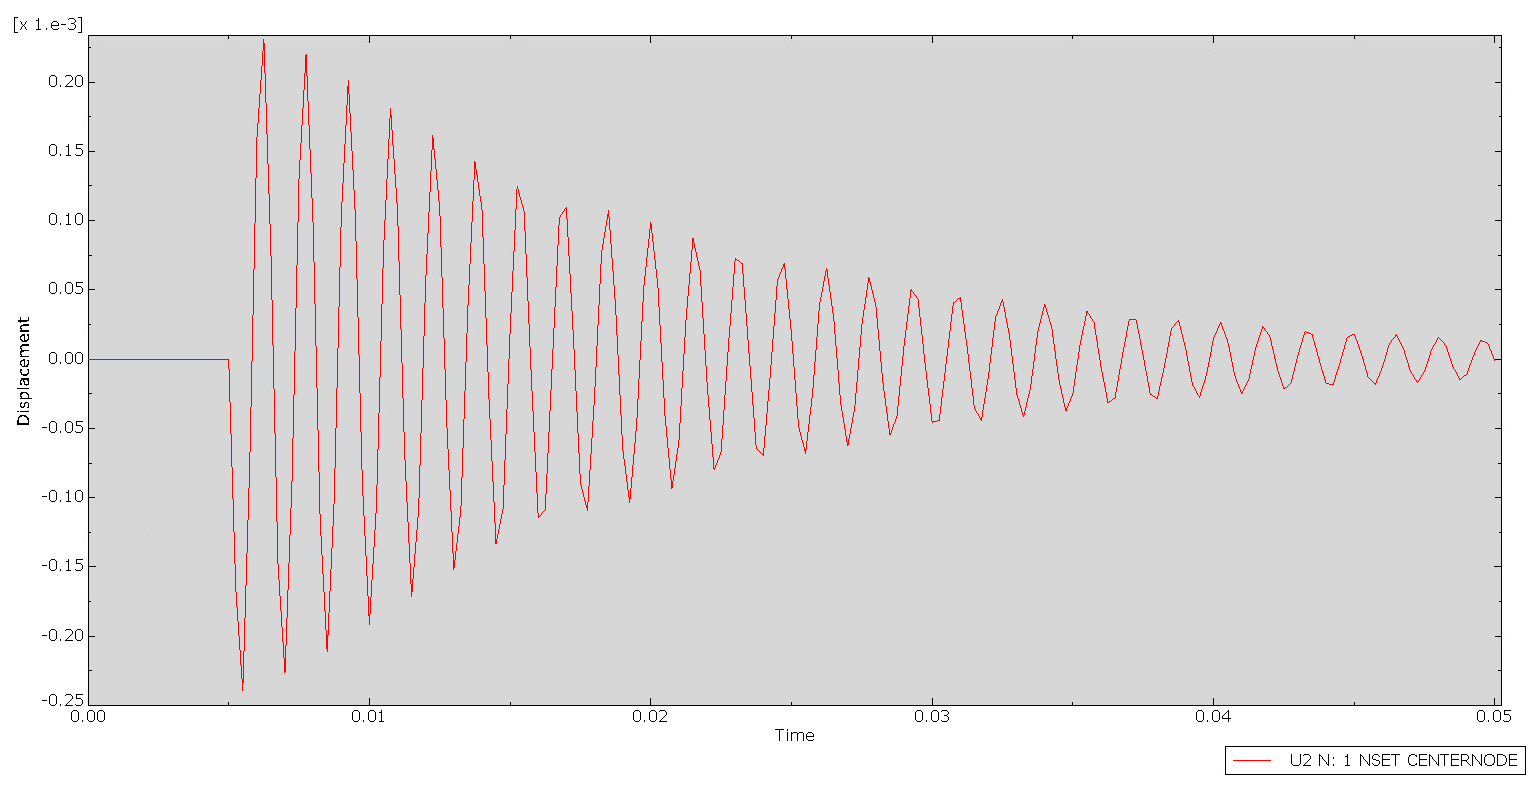
\includegraphics[width=6in]{Figures/Midpoint_U2displacement.png}
		\caption{Time-series displacement of beam midpoint.}
		\label{fig:displacement}
	\end{figure}
	
\end{document}
